\section{Erste Städte}

\begin{myexercise}
Vervollständigen Sie folgende Tabelle zu den Entstehungsgründen von Städten:
\begin{table}[H]
\centering
%\setlength\extrarowheight{25pt}
\begin{tabular}{@{}cm{2.7cm}|m{5cm}|m{6cm}@{}}
&\textbf{Theorie}             & \textbf{Entstehungsgrund}                & \textbf{Charakteristische\newline Merkmale}                                                                               \\ \midrule\midrule
\emoji{potable-water}& Hydraulisch && \\[50pt] \midrule
\emoji{church}& Theologisch &&\\[50pt] \midrule
\emoji{money-mouth-face}& Ökonomisch &&\\[50pt] \midrule
\emoji{military-helmet}& Militärisch && \\[50pt]
\end{tabular}
\caption{Theorien zur Stadtgründung und ihre Merkmale \cite{westermann}}
\label{tab:theorien}
\end{table}

\begin{myanswer}
\begin{table}[H]
\centering
\begin{tabular}{@{}p{2.5cm}|p{4.5cm}|p{5.5cm}@{}}
\textbf{Theorie}             & \textbf{Entstehungsgrund}                & \textbf{Charakteristische Merkmale}                                                                               \\ \midrule\midrule
Hydraulische Theorie         & Verfügbarkeit von Wasser                 & Stadtgründung an Quellen und Flüssen zur Organisation einer Bewässerungswirtschaft, zur Versorgung mit Trinkwasser und für bestimmte handwerkliche Arbeiten \\ \midrule
Theologische Theorie         & Existenz eines zentralen, räumlich fixierten Heiligtums & Versorgung der Priester an einem heiligen Ort durch eine größere Bevölkerungsgruppe                                \\ \midrule
Ökonomische Theorie          & Wachstum von Handel und Markt            & Kaufmannssiedlungen entlang der Handelsrouten zur Versorgung, zum Rasten und zum Schutz der Händler                \\ \midrule
Militärische Theorie         & Sicherheit und Schutz vor feindlichen Übergriffen & Verteidigung der Errungenschaften durch eine natürliche Schutzlage in der Landschaft oder durch eine errichtete Verteidigungsanlage (Mauer) \\
\end{tabular}
\caption{Theorien zur Stadtgründung und ihre Merkmale \cite{westermann}}
\label{tab:theorien-sol}
\end{table}
\end{myanswer}
\end{myexercise}

\begin{myexercise}
Vervollständigen Sie untenstehende Tabelle zu historischen Stadttypen (im Verlaufe des Unterrichts)
\end{myexercise}
\begin{table}[H]
\centering
%\setlength\extrarowheight{25pt}
\footnotesize
\begin{tabular}{m{3.5cm}|m{5.5cm}|m{5.5cm}}
\textbf{Entwicklungs-Phasen} & \textbf{Siedlungsmittelpunkt} & \textbf{Charakteristische Merkmale} \\
\midrule\midrule
\textbf{Römerzeit} \newline (200 v. Chr. bis ca. Mitte des 5. Jh.) \newline 
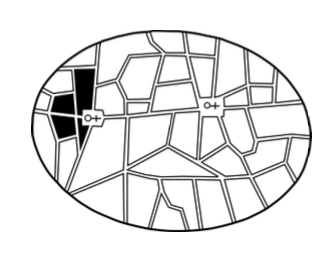
\includegraphics[width=2.5cm, height=2.5cm]{Geografie/Stadtgeografie/Figures/grundrissMittelalter}&
\begin{itemize}
\item Forum
\end{itemize} &
%\begin{itemize}
%\item Legionslager
%\item Meist rechteckiger Grundriss mit Stadtmauer
%\item zwei Hauptstrassen kreuzen sich rechtwinklig und teilen die Stadt in vier Teile (Quartiere, Viertel)
%\item Wohnblocks schachbrettartige angeordnet
%\item Amphitheater, Zirkus und Bäder
%\end{itemize}
\\
\midrule
\textbf{Mittelalter} \newline (8. bis 15. Jahrhundert)\newline 
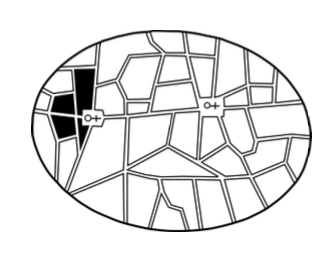
\includegraphics[width=2.5cm, height=2.5cm]{Geografie/Stadtgeografie/Figures/grundrissMittelalter} &
\begin{itemize}
\item Marktplatz / Rathaus 
\item Kirche / Kloster 
\item Burg  
\end{itemize}
&
%\begin{itemize}
%\item enge, verwinkelte Strassen, starke Überbau-
%ung
%\item Hauptverkehrsachsen laufen auf zentralen Punkt zu
%\item geschlossene, abgegrenzte Einheit
%\item Stadtmauer (oft mit Graben), Stadttore
%\item Arbeits- und Wohnstätten sehr eng miteinander verbunden (in einem Haus)
%\end{itemize}
\\
\midrule
\textbf{Renaissance / Absolutismus} \newline (16. bis 18. Jahrhundert) \newline 
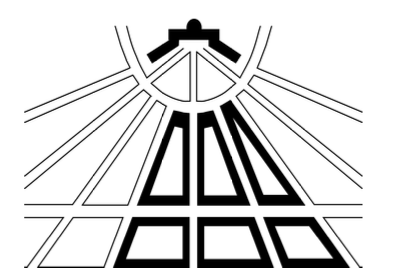
\includegraphics[width=2.5cm, height=2.5cm]{Geografie/Stadtgeografie/Figures/grundrissAbsolut}&
\begin{itemize}
\item Schlossanlage
\item Residenz (als geometrischer Mittelpunkt) 
\end{itemize} &
%\begin{itemize}
%\item planmässige Anlage (geometrische Form)
%\item Hauptachsen auf die Residenz ausgerichtet
%\item Park- und Gartenanlagen in geometrischer Form
%\item Alleen (Strassen mit Baumreihen)
%\item Vaubansche Festungswerke (mit vielen Winkeln vorgetriebenen Bastionen für den Flankenschutz)
%\end{itemize}
\\
\midrule
\textbf{Industrialisierung} \newline (19. Jahrhundert)\newline 
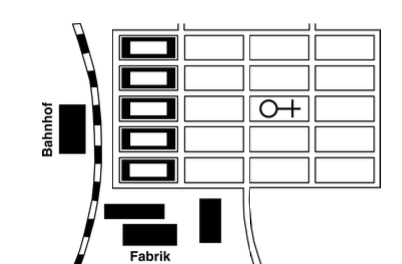
\includegraphics[width=2.5cm, height=2.5cm]{Geografie/Stadtgeografie/Figures/grundrissIndustrie} &
\begin{itemize}
\item Fabrik 
\item Bahnhof
\end{itemize}&
%\begin{itemize}
%\item rasterförmiges Strassennetz
%\item Blockrandbebauung, Häuser grenzen an die
%Strassen
%\item Blockinnenflächen oft durch Hinterhäuser
%überbaut
%\item innerstädtische Parks
%\item weitgehend räumliche Trennung von Wohnen
%und Arbeiten (aber noch enges Nebeneinan-
%der)
%\end{itemize}
\\
\midrule
\textbf{Gegenwart} \newline (20./21. Jahrhundert)\newline 
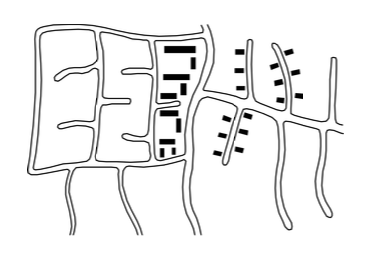
\includegraphics[width=2.5cm, height=2.5cm]{Geografie/Stadtgeografie/Figures/grundrissModern} &
\begin{itemize}
\item Einkaufszentrum
\end{itemize} &
%\begin{itemize}
%\item hierarchisch angelegtes Strassennetz:
%Hauptstrassen, Nebenstrassen, Sackgassen
%\item lockere Bebauung: Einzel- und Reihenhäu-
%ser, Punkt- und Zeilenbebauung
%\item Baugruppen
%\item hoher Grünflächenanteil
%\item klare räumliche Trennung von Wohnen und
%Arbeiten
%\end{itemize}
\\
\end{tabular}
\end{table}


\section{Die römische Stadt}
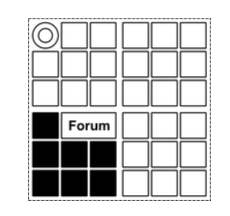
\includegraphics[width=.2\linewidth]{Geografie/Stadtgeografie/Figures/grundrissRom}
\begin{figure}[H]
\centering

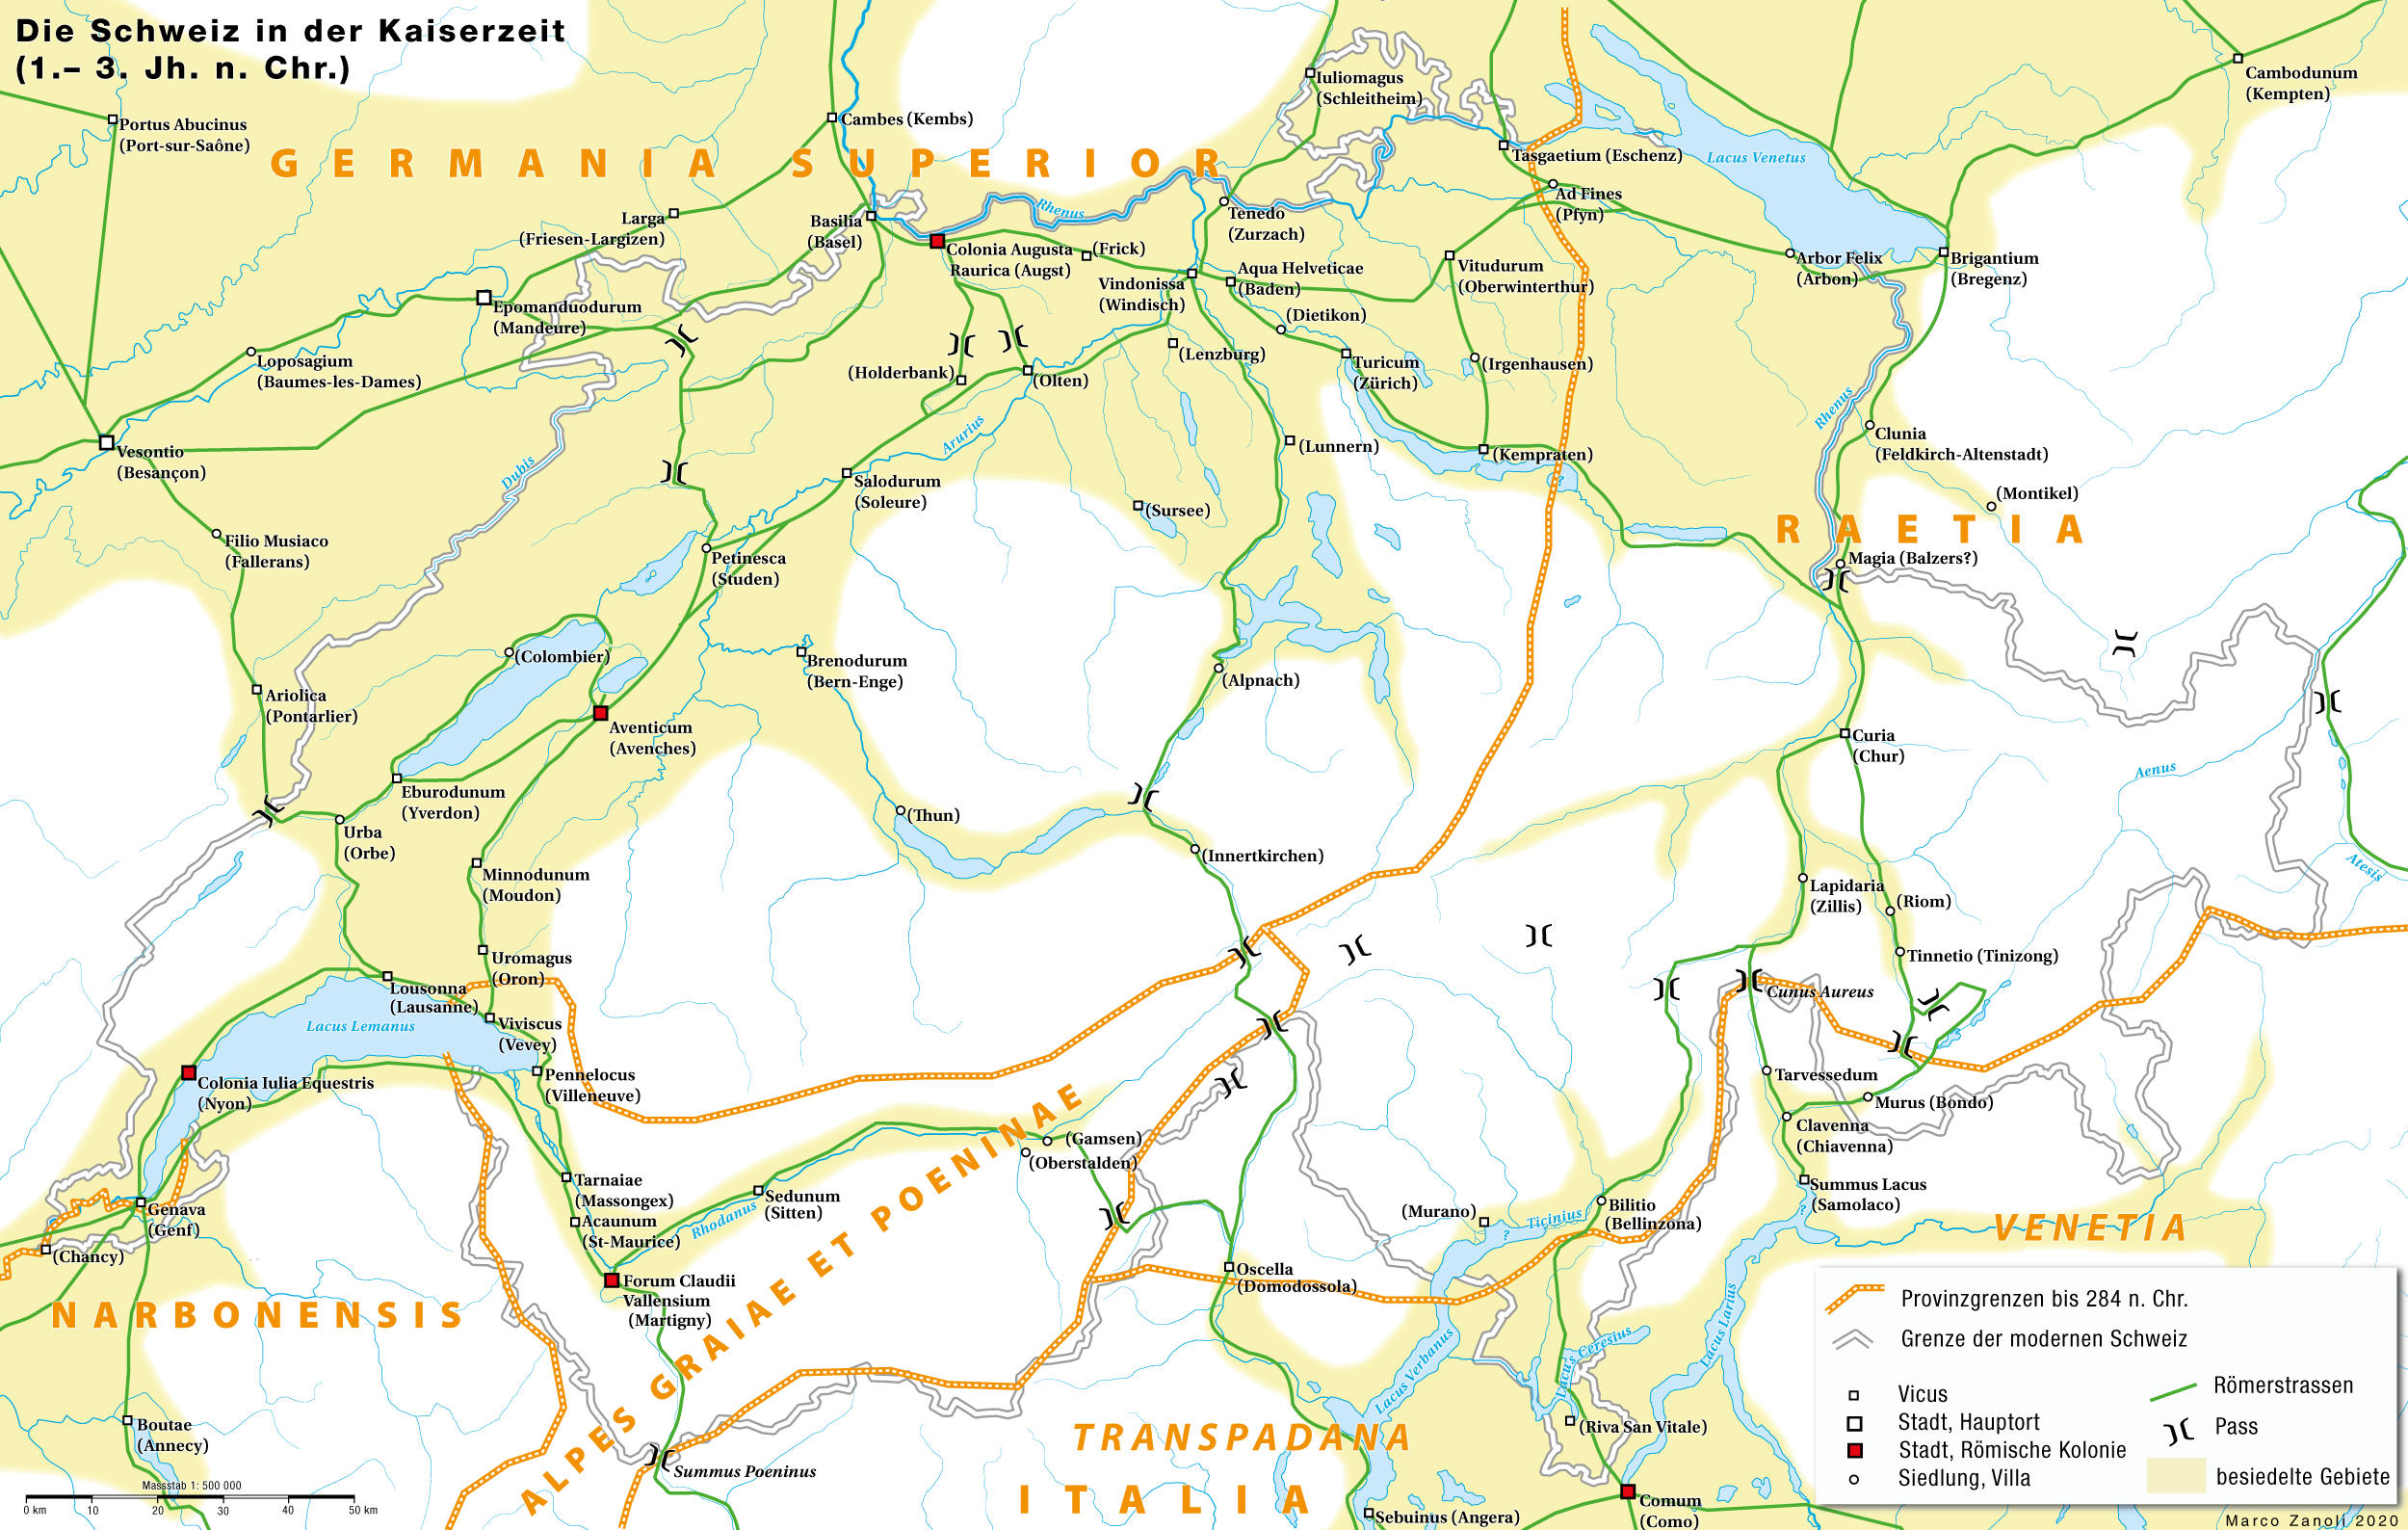
\includegraphics[width=\linewidth]{Geografie/Stadtgeografie/Figures/roemerKarte}

\caption{Römische Siedlungen in der Schweiz (1.-3. Jh. n. Chr.)}
\end{figure}
\begin{multicols}{2}
Charakteristische Mermale:
\notiz{7}
\columnbreak
\begin{figure}[H]
\centering
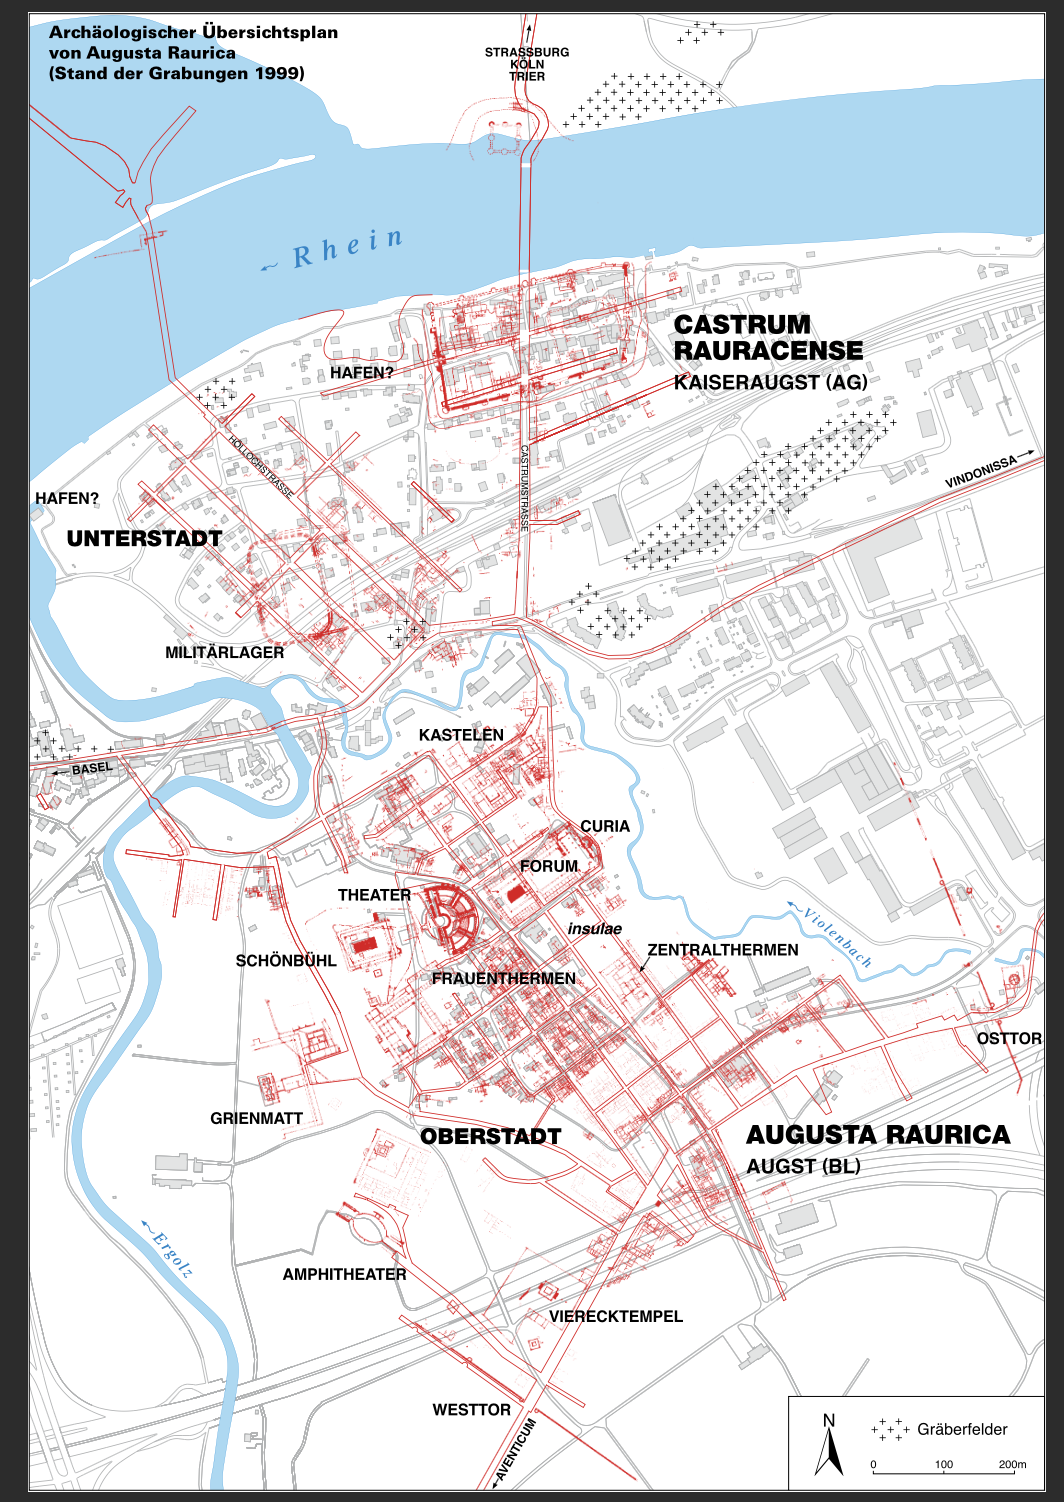
\includegraphics[width=.6\linewidth]{Geografie/Stadtgeografie/Figures/augustaRaurica}
\caption{Grundriss der Stadt Augusta Raurica}
\end{figure}

\end{multicols}


\section{Die mittelalterliche Stadt}
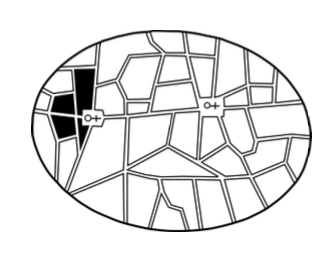
\includegraphics[width=.2\linewidth]{Geografie/Stadtgeografie/Figures/grundrissMittelalter}
\begin{myexercise}
Schauen Sie sich \href{https://www.youtube.com/watch?v=rCFdfhIiCx4}{dieses Video} an und machen Sie sich zu folgenden Fragen notizen:
\begin{itemize}
\item \textbf{Zweck}: Weshalb wurde die mittelalterliche Stadt erbaut?
\item \textbf{Struktur}: Wie ist die mittelalterliche Stadt aufgebaut?
\item \textbf{Bewohner}: Weshalb nennen sich die Stadtbewohner „Bürger“?
\item Wie unterscheiden sich Stadt- und Landbewohner?
\item Wie orientiert man sich in der Stadt?
\end{itemize}
\end{myexercise}
Charakteristische, räumliche Mermale:
\notiz{5}

\section{Die Residenzstadt}
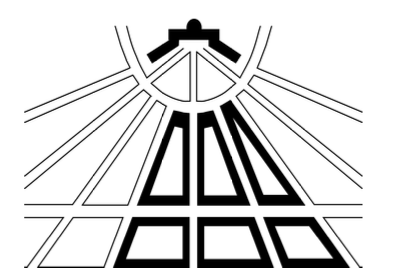
\includegraphics[width=.2\linewidth]{Geografie/Stadtgeografie/Figures/grundrissAbsolut}
\notiz{4}

\section{Die industrielle Stadt}
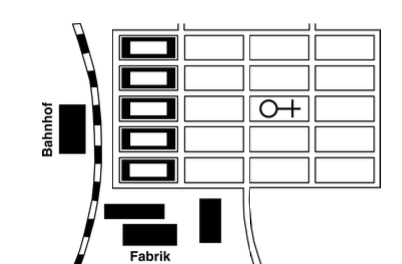
\includegraphics[width=.2\linewidth]{Geografie/Stadtgeografie/Figures/grundrissIndustrie}
\notiz{6}

\section{Die neue Stadt (``\textit{ville nouvelle}'')}
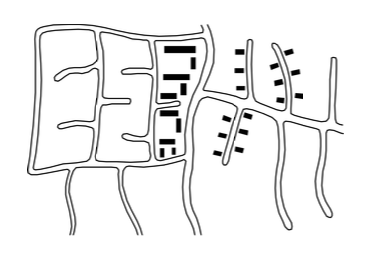
\includegraphics[width=.2\linewidth]{Geografie/Stadtgeografie/Figures/grundrissModern}
\notiz{6}

\section{Die gegenwärtige, europäische Stadt}
\notiz{6}

\begin{myexercise}
Vervollständigen Sie folgende Grafik:
\begin{figure}[H]
\centering
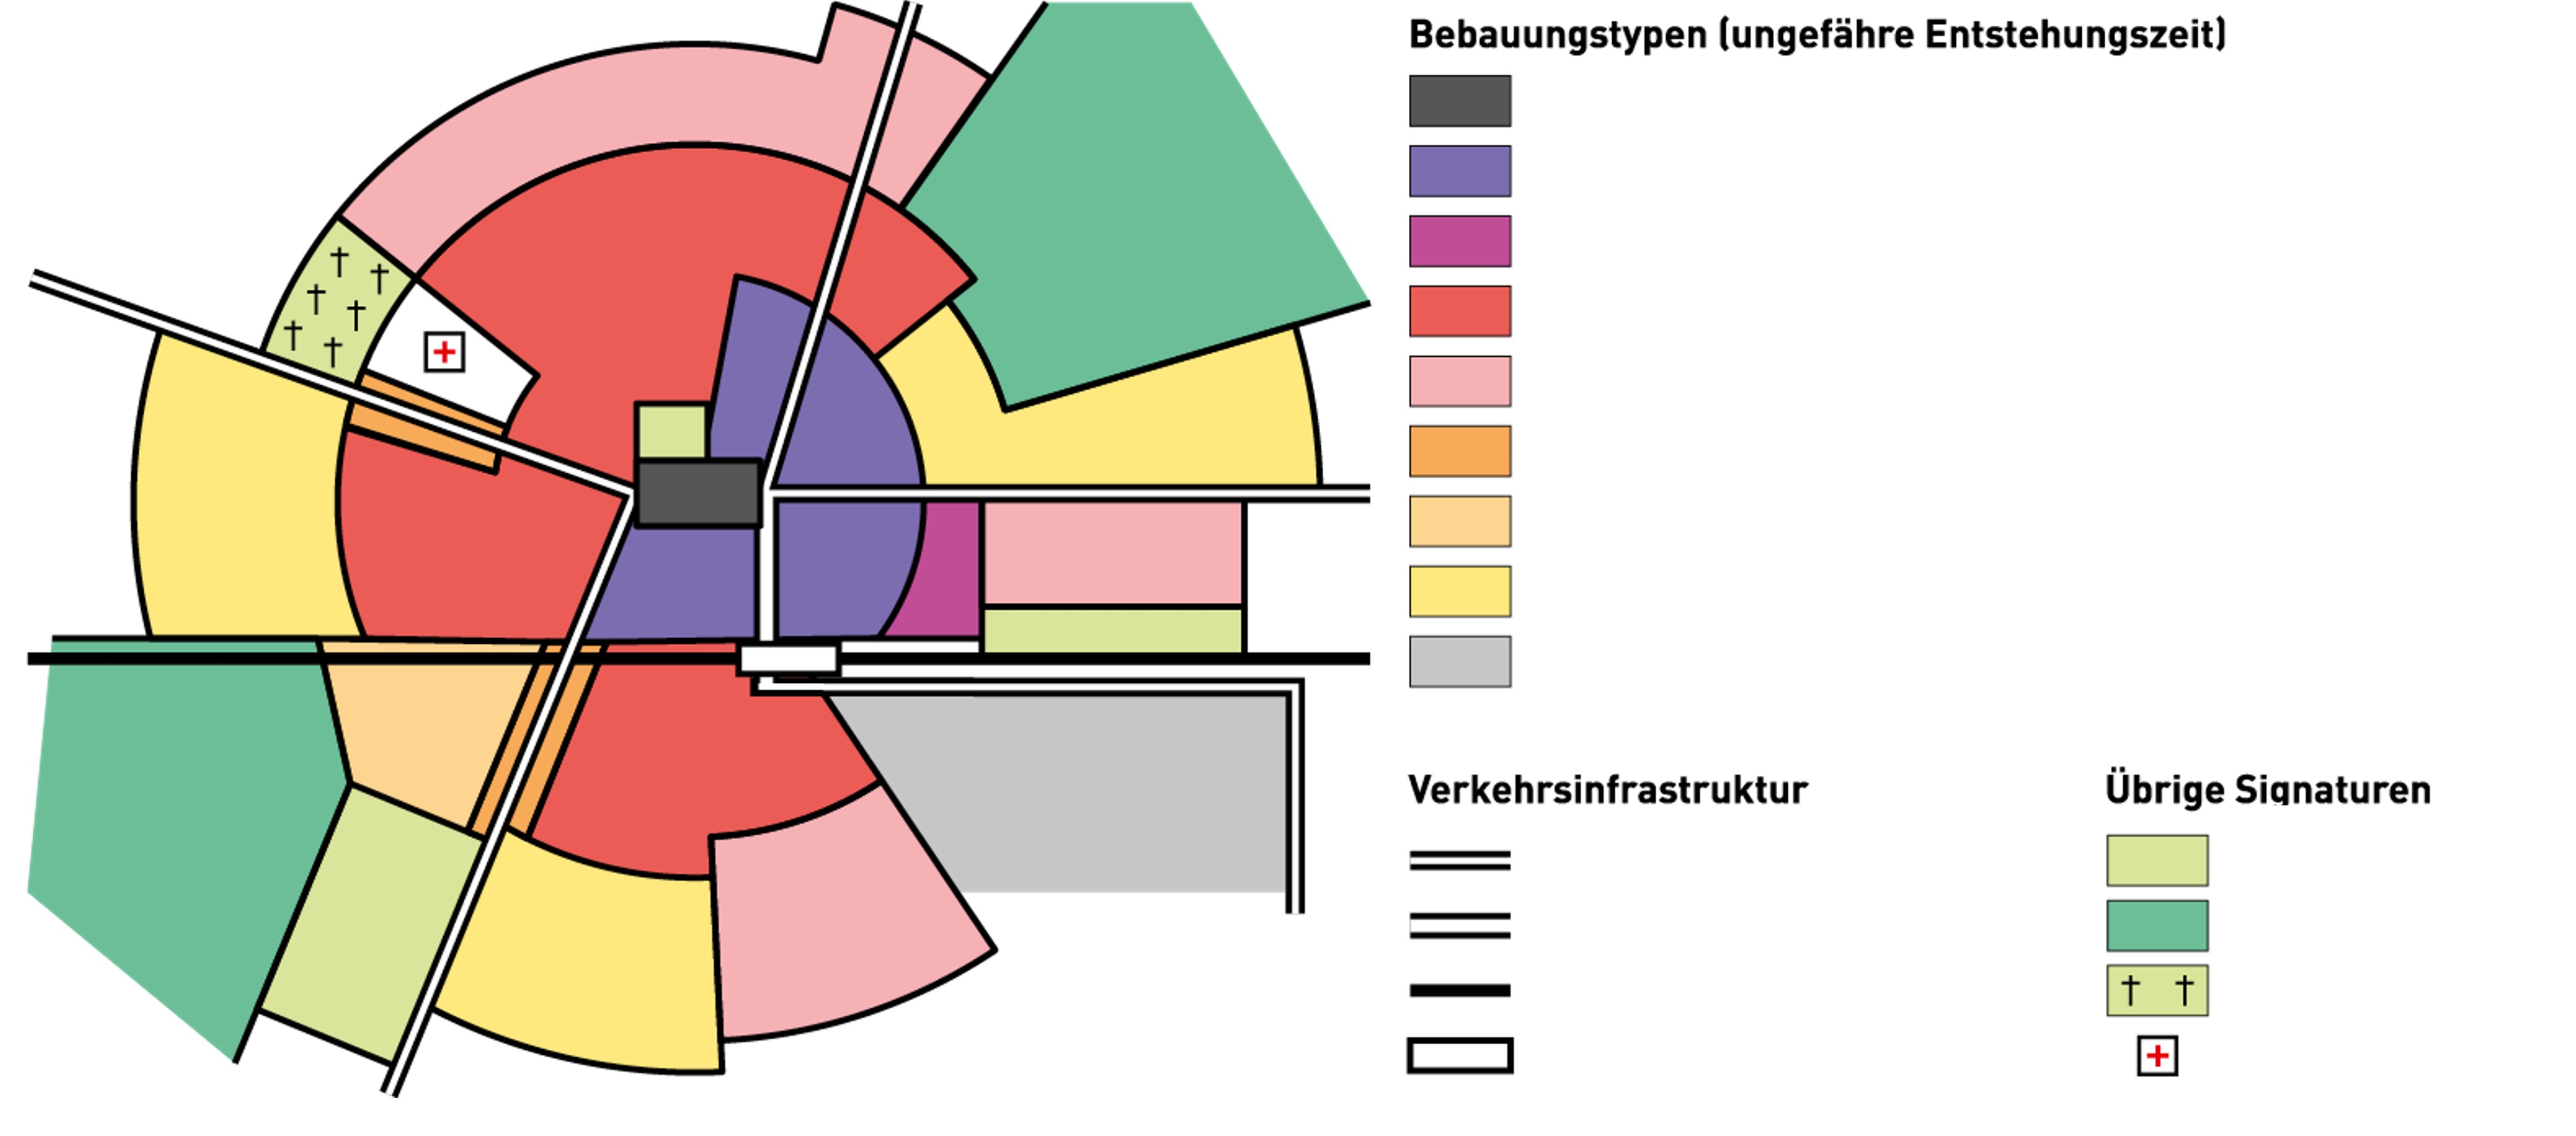
\includegraphics[width=\linewidth]{Geografie/Stadtgeografie/Figures/EuropaeischeStadtModellLeer}
\end{figure}
\begin{myanswer}
\begin{figure}[H]
\centering
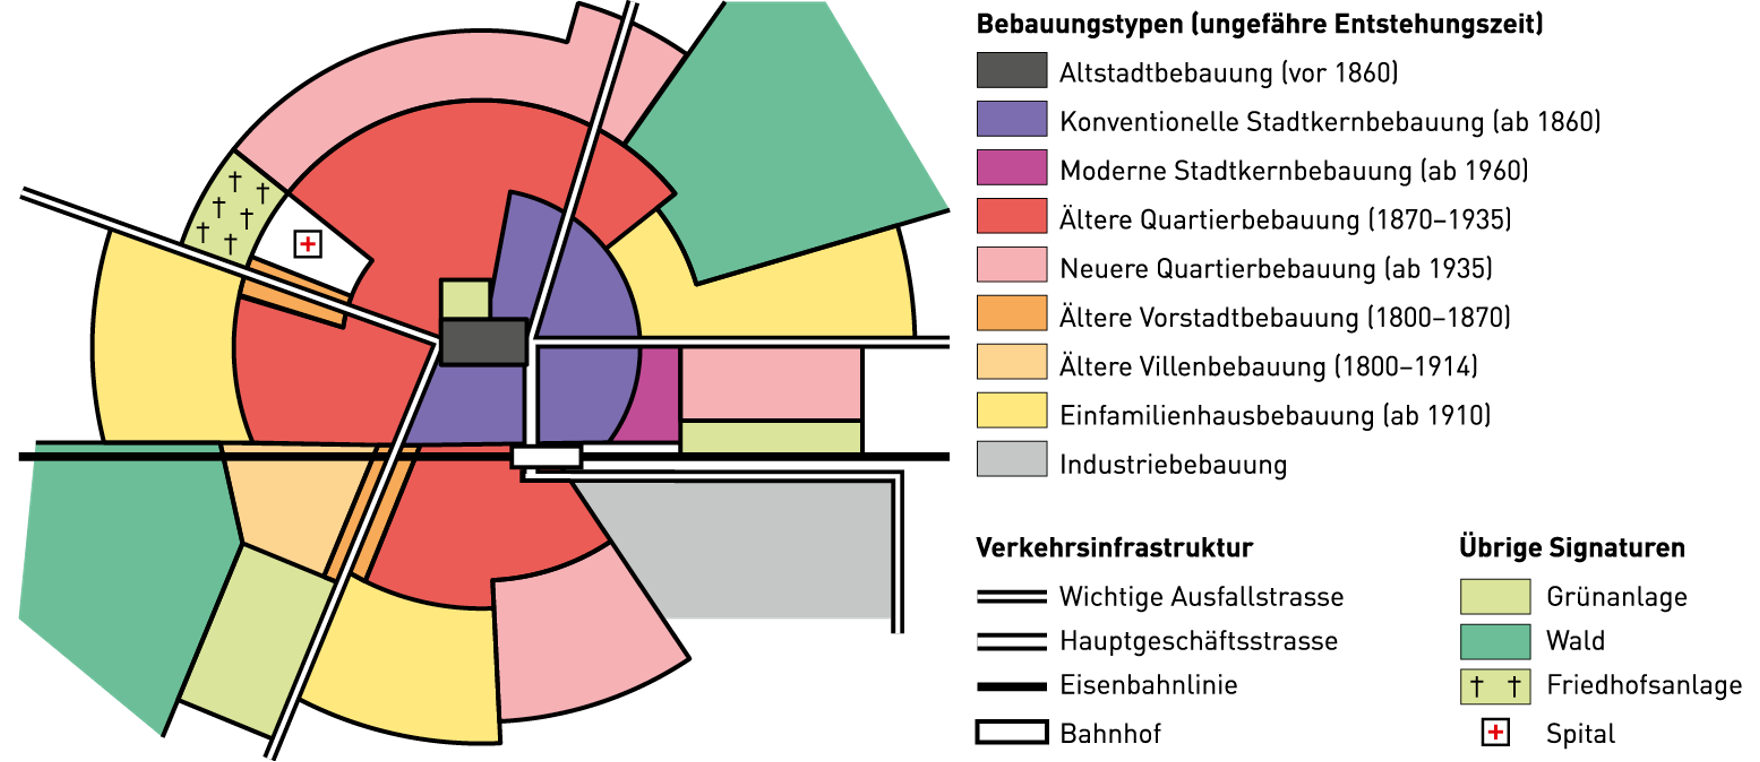
\includegraphics[width=\linewidth]{Geografie/Stadtgeografie/Figures/EuropaeischeStadtModell}
\end{figure}
\end{myanswer}
\end{myexercise}


\begin{myexercise}
Städtebauperioden lassen sich im Grundriss einer Stadt erkennen. Aufgrund von Stadterweiterungen können im Laufe der Zeit häufig mehrere Stadtentwicklungsphasen in einer Stadt gefunden werden. Es kann aber durchaus sein, dass aus bestimmten Gründen die eine oder andere Stadtentwicklungsphase nicht mehr erkennbar ist.

Betrachten Sie mit Hilfe von \href{https://www.google.com/earth}{Google Earth} die Grundrisse ausgewählter Städte.

Nennen Sie die erkennbare Stadtentwicklungsphase bei den aufgeführten Stadtteilen (z.B. Stadtzentrum) und notieren Sie in Stichworten die Merkmale, welche auf diese Stadtentwicklungsphase hindeuten.
\begin{table}[H]
\setlength\extrarowheight{25pt}
\footnotesize
\centering
\begin{tabular}{p{3.9cm}|p{5.1cm}|p{6cm}}
\textbf{Städte und Stadtteile} & \textbf{Stadtentwicklungsphasen} & \textbf{Merkmale} \\ \midrule\midrule
\multirow{2}{*}{\shortstack[l]{\textbf{1. Nördlingen (DE)}\\ 1A: Stadtzentrum\\
1B: Talbreite (Quartier)}} & 1A: & \\ \cline{2-3}
& 1B: & \\ \midrule
\multirow{2}{*}{\shortstack[l]{\textbf{2. Arles (FR)}\\2A: Stadtzentrum\\
2B: Avenue de Jerez}} & 2A: & \\ \cline{2-3}
& 2B: & \\ \midrule
\multirow{2}{*}{\shortstack[l]{\textbf{3. Palmanova (IT)}\\3A: Stadtzentrum\\
3B: Outlet Village}} & 3A: &\\ \cline{2-3}
& 3B: & \\ \midrule
\multirow{2}{*}{\shortstack[l]{\textbf{4. Mannheim (DE)}\\4A: Stadtzentrum\\
4B: Gartenstadt (Quartier)}} & 4A: & \\ \cline{2-3}
& 4B: & \\ \midrule
\multirow{2}{*}{\shortstack[l]{\textbf{5. Lyon (FR)}\\5A: Lugdunum ($\rightarrow$ Ruinen)\\5B: 6. Arrondissement}} & 5A & \\ \cline{2-3}
& 5B: & \\ \midrule
\multirow{2}{*}{\shortstack[l]{\textbf{6. Winterthur (CH)}\\6A: Stadtzentrum\\6B: Sulzerareal}} & 6A: &\\ \cline{2-3}
& 6B: & \\
%\textbf{7. Stadt der Exkursion (irgendwo in Europa)} & 7A: ... & ... \\ \cline{2-3}
%& 7B: ... & ... \\ \midrule
\end{tabular}
\end{table}

\begin{myanswer}
\begin{table}[H]
\centering
\begin{tabular}{p{4cm}|p{4cm}|p{5cm}}
\textbf{Städte} & \textbf{Stadtentwicklungsphasen} & \textbf{Merkmale} \\ \midrule\midrule
\textbf{1. Nördlingen (DE)} & 1A: Mittelalter & Stadtmauer, verwinkelte Straßen, starke Überbauung \\ \cline{2-3}
& 1B: Gegenwart & Einzel- und Reihenhäuser mit Gärten, Quartierstraßen \\ \midrule
\textbf{2. Arles (FR)} & 2A: Römerzeit / Mittelalter & Amphitheater, Theater, Stadtmauer, enge verwinkelte Straßen \\ \cline{2-3}
& 2B: Gegenwart & Einkaufszentren, Parkplätze \\ \midrule
\textbf{3. Palmanova (IT)} & 3A: Renaissance/Absolutismus & sternförmige Festungsanlagen, Schanzen \\ \cline{2-3}
& 3B: Gegenwart & Einkaufszentrum, Parkplätze \\ \midrule
\textbf{4. Mannheim (DE)} & 4A: Renaissance/Absolutismus & Barockschloss, planmäßige Anlage, geometrische Form \\ \cline{2-3}
& 4B: Gegenwart & Einzel- und Reihenhäuser mit Gärten, Quartierstraßen, Baugruppen \\ \midrule
\textbf{5. Lyon (FR)} & 5A: Römerzeit & Theater, Odeon \\ \cline{2-3}
& 5B: Industrialisierung & rasterförmiges Straßennetz, Blockrandbebauung, Stadtpark \\ \midrule
\textbf{6. Winterthur (CH)} & 6A: Mittelalter & verwinkelte Straßen, starke Überbauung \\ \cline{2-3}
& 6B: Industrialisierung & Fabrikanlagen \\
%\textbf{7. Stadt der Exkursion (irgendwo in Europa)} & 7A: ... & ... \\ \cline{2-3}
%& 7B: ... & ... \\ \midrule
\end{tabular}
\end{table}
\end{myanswer}
\end{myexercise}



\section{Anhang: Übersicht Städte-Entwicklungsphasen in Europa}
\begin{table}[H]
\centering
\footnotesize
\begin{tabular}{p{3.5cm}|p{4.5cm}|p{7cm}}
\textbf{Entwicklungs-Phasen} & \textbf{Siedlungsmittelpunkt} & \textbf{Charakteristische Merkmale} \\
\midrule\midrule
\textbf{Römerzeit} \newline (200 v. Chr. bis ca. Mitte des 5. Jh.) \newline 
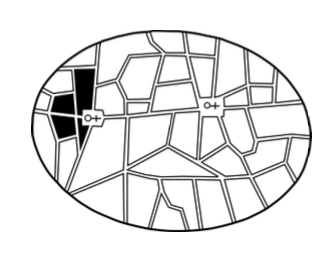
\includegraphics[width=2.5cm, height=2.5cm]{Geografie/Stadtgeografie/Figures/grundrissMittelalter}&
\begin{itemize}
\item Forum
\end{itemize} &
\begin{itemize}
\item Legionslager
\item Meist rechteckiger Grundriss mit Stadtmauer
\item zwei Hauptstrassen kreuzen sich rechtwinklig und teilen die Stadt in vier Teile (Quartiere, Viertel)
\item Wohnblocks schachbrettartige angeordnet
\item Amphitheater, Zirkus und Bäder
\end{itemize}
\\
\midrule
\textbf{Mittelalter} \newline (8. bis 15. Jahrhundert)\newline 
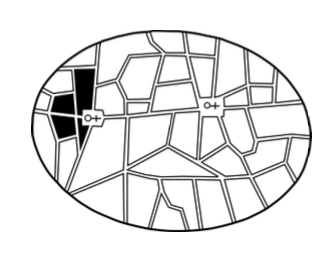
\includegraphics[width=2.5cm, height=2.5cm]{Geografie/Stadtgeografie/Figures/grundrissMittelalter} &
\begin{itemize}
\item Marktplatz / Rathaus 
\item Kirche / Kloster 
\item Burg  
\end{itemize}
&
\begin{itemize}
\item enge, verwinkelte Strassen, starke Überbauung
\item Hauptverkehrsachsen laufen auf zentralen Punkt zu
\item geschlossene, abgegrenzte Einheit
\item Stadtmauer (oft mit Graben), Stadttore
\item Arbeits- und Wohnstätten sehr eng miteinander verbunden (in einem Haus)
\end{itemize}
\\
\midrule
\textbf{Renaissance /\newline Absolutismus} \newline (16. bis 18. Jahrhundert) \newline 
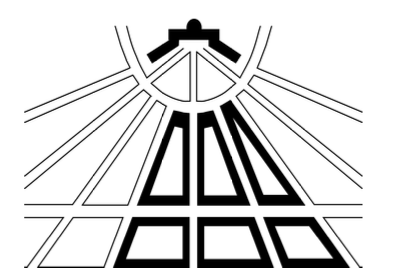
\includegraphics[width=2.5cm, height=2.5cm]{Geografie/Stadtgeografie/Figures/grundrissAbsolut}&
\begin{itemize}
\item Schlossanlage
\item Residenz (als geometrischer Mittelpunkt) 
\end{itemize} &
\begin{itemize}
\item planmässige Anlage (geometrische Form)
\item Hauptachsen auf die Residenz ausgerichtet
\item Park- und Gartenanlagen in geometrischer Form
\item Alleen (Strassen mit Baumreihen)
\item Vaubansche Festungswerke (mit vielen Winkeln vorgetriebenen Bastionen für den Flankenschutz)
\end{itemize}
\\
\midrule
\textbf{Industrialisierung} \newline (19. Jahrhundert)\newline 
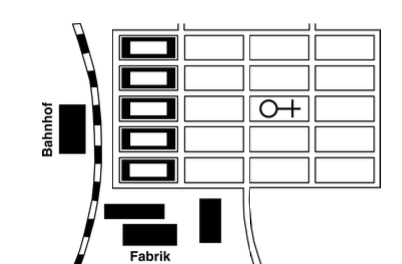
\includegraphics[width=2.5cm, height=2.5cm]{Geografie/Stadtgeografie/Figures/grundrissIndustrie} &
\begin{itemize}
\item Fabrik 
\item Bahnhof
\end{itemize}&
\begin{itemize}
\item rasterförmiges Strassennetz
\item Blockrandbebauung, Häuser grenzen an die Strassen
\item Blockinnenflächen oft durch Hinterhäuser überbaut
\item innerstädtische Parks
\item weitgehend räumliche Trennung von Wohnen
und Arbeiten (aber noch enges Nebeneinander)
\end{itemize}
\\
\midrule
\textbf{Gegenwart} \newline (20./21. Jahrhundert)\newline 
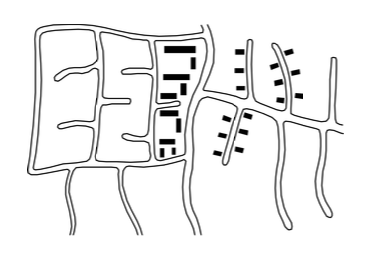
\includegraphics[width=2.5cm, height=2.5cm]{Geografie/Stadtgeografie/Figures/grundrissModern} &
\begin{itemize}
\item Einkaufszentrum
\end{itemize} &
\begin{itemize}
\item hierarchisch angelegtes Strassennetz: Hauptstrassen, Nebenstrassen, Sackgassen
\item lockere Bebauung: Einzel- und Reihenhäuser, Punkt- und Zeilenbebauung
\item Baugruppen
\item hoher Grünflächenanteil
\item klare räumliche Trennung von Wohnen und Arbeiten
\end{itemize}
\\
\end{tabular}
\caption{Übersicht Städte-Entwicklungsphasen in Europa}
\end{table}

\begin{mychallenge}[NZZ-Artikel zu 3D-Modell der Stadt Zürich]
\begin{figure}[H]
\centering
\colorbox{white}{\includegraphics[width=.9\linewidth]{"Geografie/Stadtgeografie/Appendix/2022-04-16 Zürich 3D-Modell"}}
\end{figure}
\end{mychallenge}


\newpage
\section{Lernziele}
\begin{todolist}
\item Ich verstehe typische räumliche Strukturen europäischer Gründunsstädte aus der Römerzeit, dem Mittelalter, der Industrialisierung und der Gegenwart. Ich kann Siedlungsmittelpunkt, Verkehrstypen und weitere charakteristische Mermale für jede der genannten Epochen auflisten und erklären
\item Ich kann die historische Entstehung einer europäischen Stadt beschreiben, indem ich die Viertel einer europäische Stadt aufgrund ihrer räumlichen Mermale einer Gründungszeit (Römer, Mittelalter, Industrialisierung oder Neuzeit) zuordne.
\item Ich kann eine europäische Stadt in Ihre typischen Bebauungstypen einordnen.
\end{todolist}

